% chapter3_11.tex -- de (German)
% install splitti79's OLED display
\section{OLED-Display einrichten}

Die {\Bezeichnung} funktioniert zwar bereits voillst�ndig, nur das
optionale OLED-Display zeigt noch nichts an. Die Anzeige im Display wird
�ber die I2C-Schnittstelle �bertragen.

Quellen:\\
\url{https://github.com/splitti/oled_phoniebox}\\
\url{https://splittscheid.de/selfmade-phoniebox/#5_3}

Auch dieses Projekt kann �ber einen sogenannten \software{one line
installer} installiert werden. Im Gegensatz zum Installer der 
{\Bezeichnung}-Soft\-ware aus Kapitel
\label{sect:phoniebox_onelineinstaller} ist der f�r die OLED-Software
%von \textbf{@splitti79}
%(\url{https://forum-raspberrypi.de/user/54710-splitti79/})
eher noobtauglich \smiley{smile}

%\verb|cd; rm o4p_installer.sh; wget https://raw.githubusercontent.com/splitti/oled_phoniebox/master/scripts/install/o4p_installer.sh; chmod +x o4p_installer.sh; ./o4p_installer.sh|
\begin{bclogo}[logo = \bclampe, noborder = true]{Hinweis}
Aus Gr�nden des Seitenlayouts wird der \textit{one line installer} in
seine Einzelbefehle zerlegt. 
\end{bclogo}

\cmdPi{cd;}\\
\cmdPi{rm o4p\_installer.sh;}\\
\cmdPi{\begin{scriptsize}wget https://raw.githubusercontent.com/splitti/oled\_phoniebox/master/scripts/install/o4p\_installer.sh;\end{scriptsize}}\\
\cmdPi{chmod +x o4p\_installer.sh;}\\
\cmdPi{./o4p\_installer.sh}\\

Auch hier zeigt eine Bilderstrecke mehr als viele Worte:

\begin{figure}[!h]
\centering
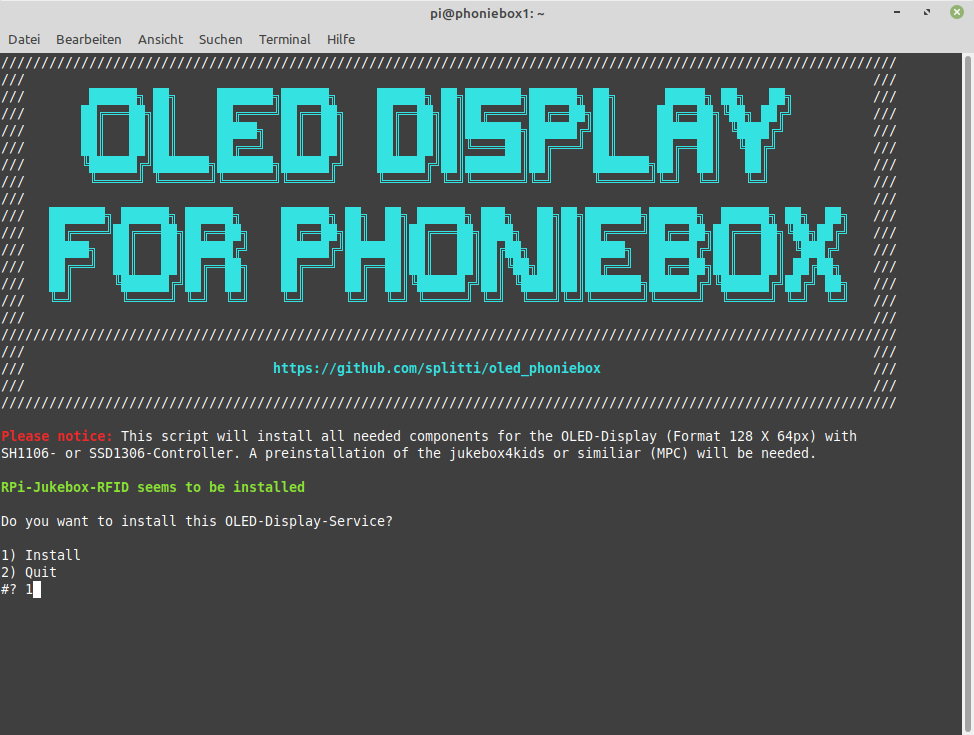
\includegraphics[width=0.47\textwidth]{/OLED/oled01.png}
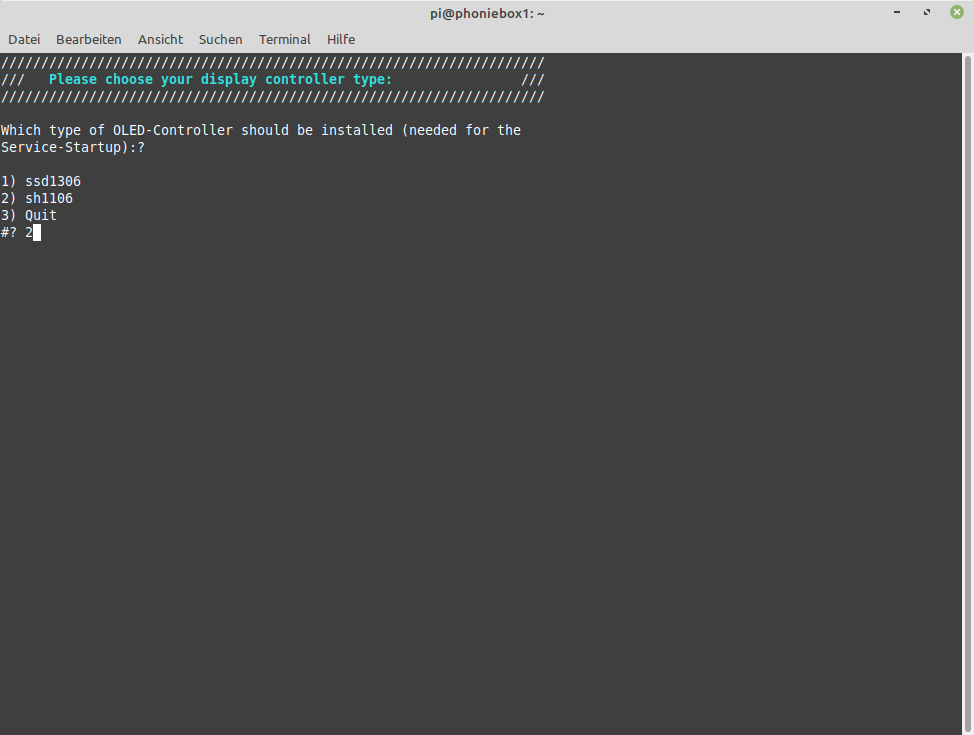
\includegraphics[width=0.47\textwidth]{/OLED/oled02.png}
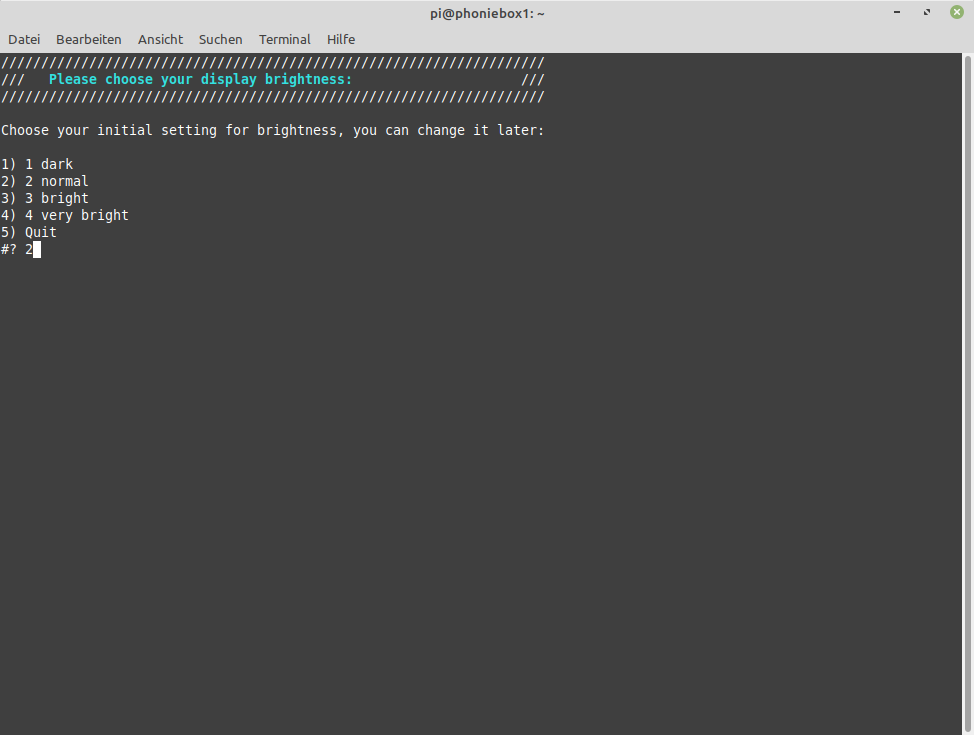
\includegraphics[width=0.47\textwidth]{/OLED/oled03.png}
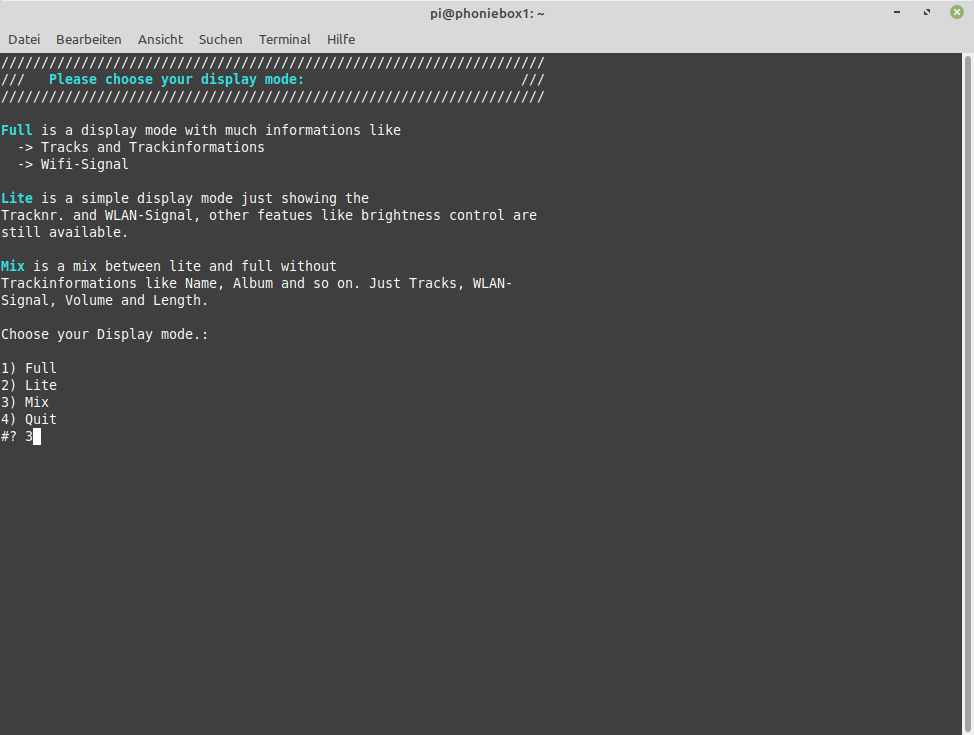
\includegraphics[width=0.47\textwidth]{/OLED/oled04.png}
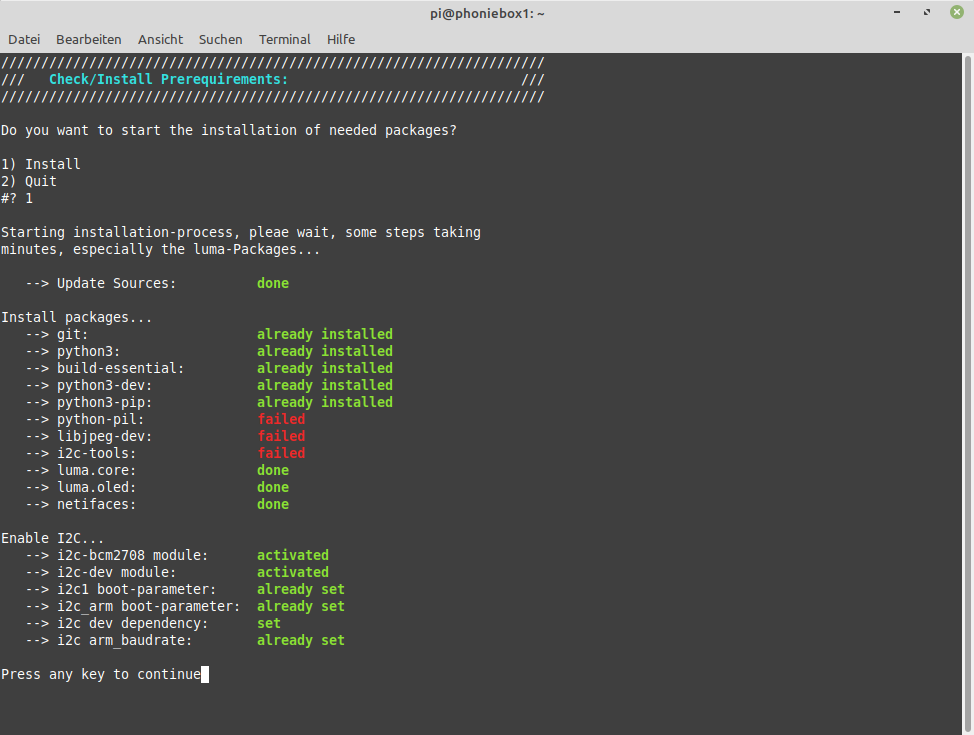
\includegraphics[width=0.47\textwidth]{/OLED/oled05.png}
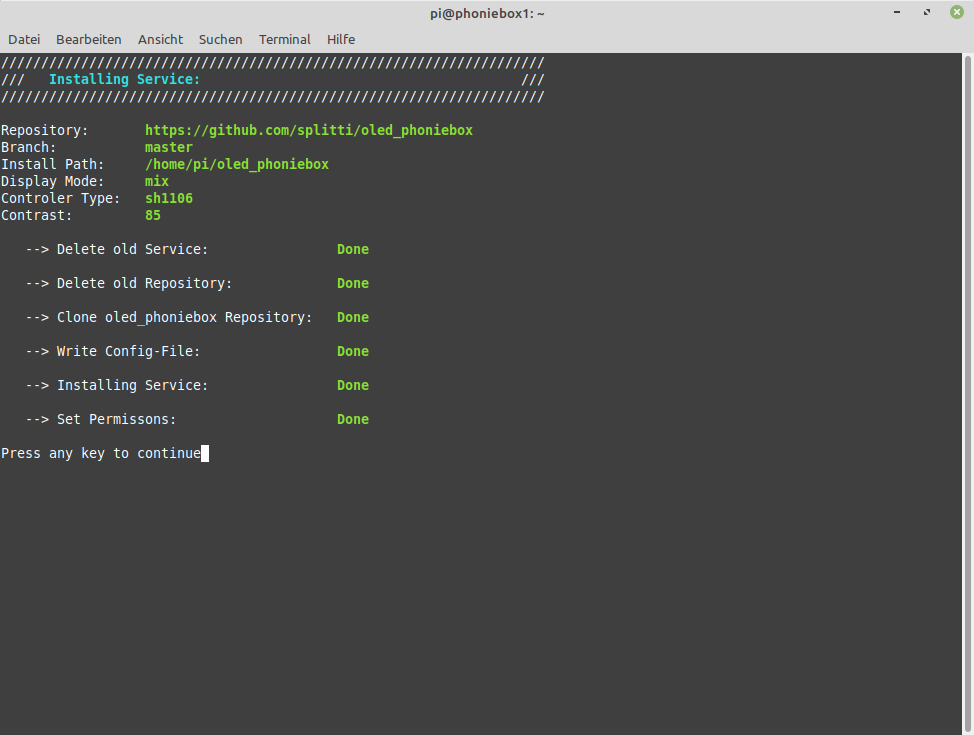
\includegraphics[width=0.47\textwidth]{/OLED/oled06.png}
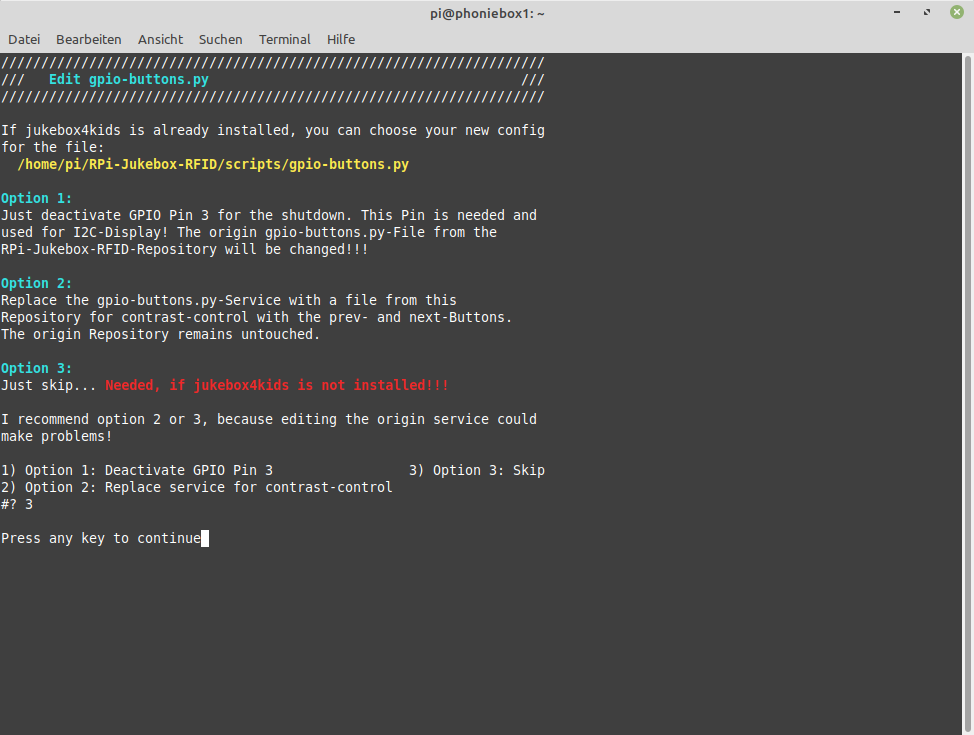
\includegraphics[width=0.47\textwidth]{/OLED/oled07.png}
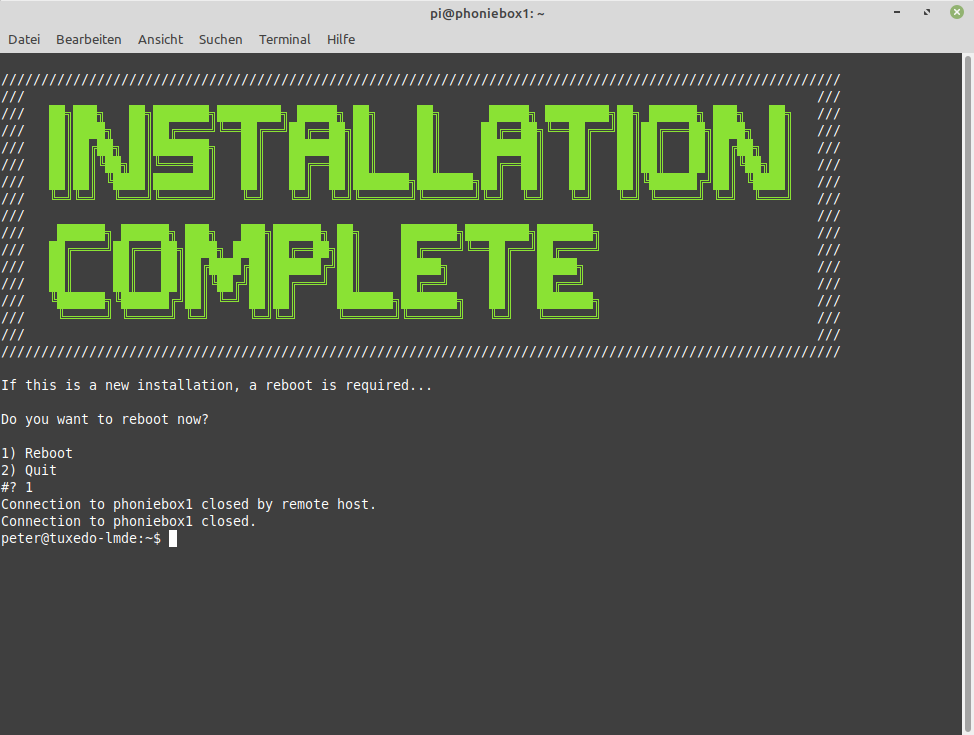
\includegraphics[width=0.47\textwidth]{/OLED/oled08.png}
\caption{splitti79s one line installer}
\end{figure}
